\section{Functional MRI} \label{sec:fMRI}

Different MRI techniques exist to accentuate particular tissue types, physiological phenomena, etc. Among these the Blood Oxygen Level Dependent (BOLD) will be described in this section. The reason for solely focusing on BOLD in this project, is due to it being the most widely used and accepted method for functional Magnetic Resonance Imaging (fMRI). BOLD is favored in mapping brain activity, because it offers a high contrast to noise ratio and it is relatively simple to implement. \cite{Lee2002}    
 
fMRI measures the metabolic changes associated with different neurological tasks in multiple brain areas. fMRI offers advantages which predominantly are high temporal and spatial resolution, low cost, and most importantly being non-invasive, which has made it a exceedingly popular method for imaging brain activity. The versatility of fMRI has made it a very important tool by being a biomarker for diseases and test of of pharmaceuticals. \cite{Glover2011} 

The physiologic background facilitating the possibility of measuring brain activity through the BOLD contrast is found in the local metabolism during neural activation. Multiple steps in forming and transmitting a neurological signal requires adenosine triphosphate (ATP) consumption e.g. reception and reformation of an action potential. When activating a brain area in e.g. finger tapping, the ATP starts to be processed, leading to a decrease in oxygen concentration and increase in waste. Thereby the metabolic need for oxygen increases. As the movement is planned and executed, factors, which are present in the local tissue of the corresponding brain area, activate a vasodilation, increasing the blood flow to that area to reestablish the local homeostasis. During this regulation a special and not fully understood phenomenon occurs as more oxygenated blood than needed to compensate for the offset is delivered. Thereby flooding the local region with oxygenated blood. The overall increase in neural activity in that specific area following the need for metabolic regulation thereby permits blood oxygen level dependent (BOLD) contrast to studied. An example illustrating the measurable hemodynamic response can se found in \figref{fig:back:HRF}. \cite{Glover2011,Poldrack2011}

\begin{figure}[H]                 
	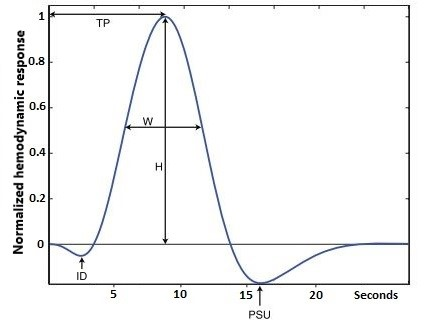
\includegraphics[width=.48\textwidth]{figures/aBackground/HRF}  
	\caption{A depiction of a single hemodynamic response curve. ID is the initial dip as less oxygen will be present as the metabolic demand increases, TP is time from stimulus until peak, W and H is the width and height of the response and PSU is a post stimulus undershoot. \cite{Poldrack2011}}
	\label{fig:back:HRF} 
\end{figure}

\Figref{fig:back:HRF} should be considered the perfect noiseless hemodynamic response curve, to a brief stimuli, though the reality is that the response is noise and delayed in time. The peak height of the curve is commonly the most interesting feature of the response, as it portrays the amount of neural activity. The time to peak will occur 4-6 seconds after stimulus onset. The duration of a response is around 20 seconds. There will further be a noticeable initial dip of 1-2 seconds duration and a 20 second poststimulus undershoot. \cite{Poldrack2011}    \\
As established above the BOLD signal is effected by the neural activity producing changes in the local blood flow, blood volume and blood oxygenation. The crucial part to why MRI can detect this natural contrast is that oxygenated hemoglobin $(HbO_2)$ is diamagnetic, and deoxygenated hemoglobin $(Hb)$ has four unpaired electrons thereby making it highly paramagnetic. Thus, the more oxygenated blood in an area, the larger the contrast compared to other brain regions would be visible in an acquired image. \cite{Glover2011,Poldrack2011,Khanna2015} \Figref{fig:back:bold} illustrates how the contrast i dependent on the amount of oxygenated hemoglobin. \cite{Glover2011}

\begin{figure}[H]                 
	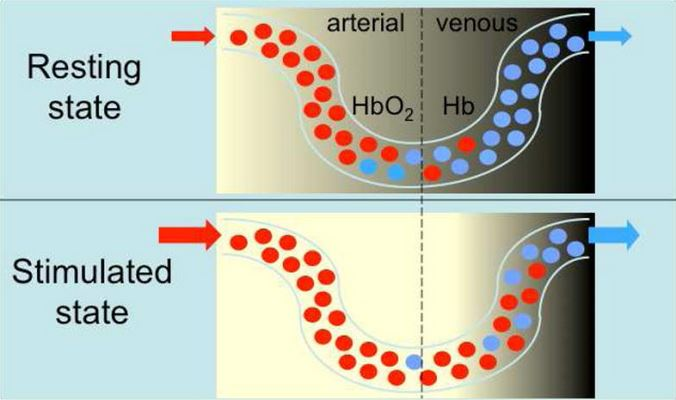
\includegraphics[width=.47\textwidth]{figures/aBackground/bold_response}  
	\caption{Illustration of how the difference in oxygen concentration in the hemoglobin change the magnetic properties, resulting in a higher measurable contrast \cite{Glover2011}.}
	\label{fig:back:bold} 
\end{figure}

This change in local magnetic properties increases the magnetic inhomogeneity, which can be recorded by using a $T2^*$ sequence, which was presented in \secref{sec:physics} \cite{Lee2002}.  
